\documentclass{article}
\usepackage{graphicx}
\usepackage[a4paper, hmargin = 2.5cm, vmargin = 2.5cm]{geometry}
\usepackage[english]{babel}

\title{Database project: Travel agency \\ (Milestone 2)}
\author{Oliver Baltisberger, Rachid Flueckiger, Christian Pernet}
\date{\today}

\begin{document}
	\maketitle
	
	\section*{Adjustment of ER-Diagram}
	Based on the feedback  we received for Milestone 1 and our discussions related to Milestone 2, we decided to slightly adjust our ER-Diagram:
	\begin{itemize}
		\item The entity Payment is no longer modeled as a weak entity. Further, we allow installment payments (e.g. clients can pay for their individualized trips with several payments), which leads to a 1:N relationship.
		This also implies that the amount of the payment can be different from the price of the trip.
		\item We added the attributes City and Country to the entity Activity. This allows us to know where an activity takes place.
		For simplicity, we decided to drop the attribute Contact from the entity Activity. The phone number of the activity provider is not essential in our simplified model.
		\item We moved the attributes Date and Number of Nights from the entities Activity, Transport and Accommodation to the relationships has\_activity, has\_transport and has\_accommodation, respectively.
		We opted for this adjustment, because Date and Number of Nights are the only things that might change, while all other attributes of these three entities cannot change between different trips (e.g. the address of a hotel always stays the same).
		This allows us to load data more efficiently into our database (e.g. when we add an activity to a trip, we only have to specify the date when the activity takes place, but not the name or description of the activity).
	\end{itemize}
	
You find our adjusted ER-Diagram on the next page.
	\newpage
	
	\section*{ER-Diagram}
	\begin{figure}[htbp]
		\centering
			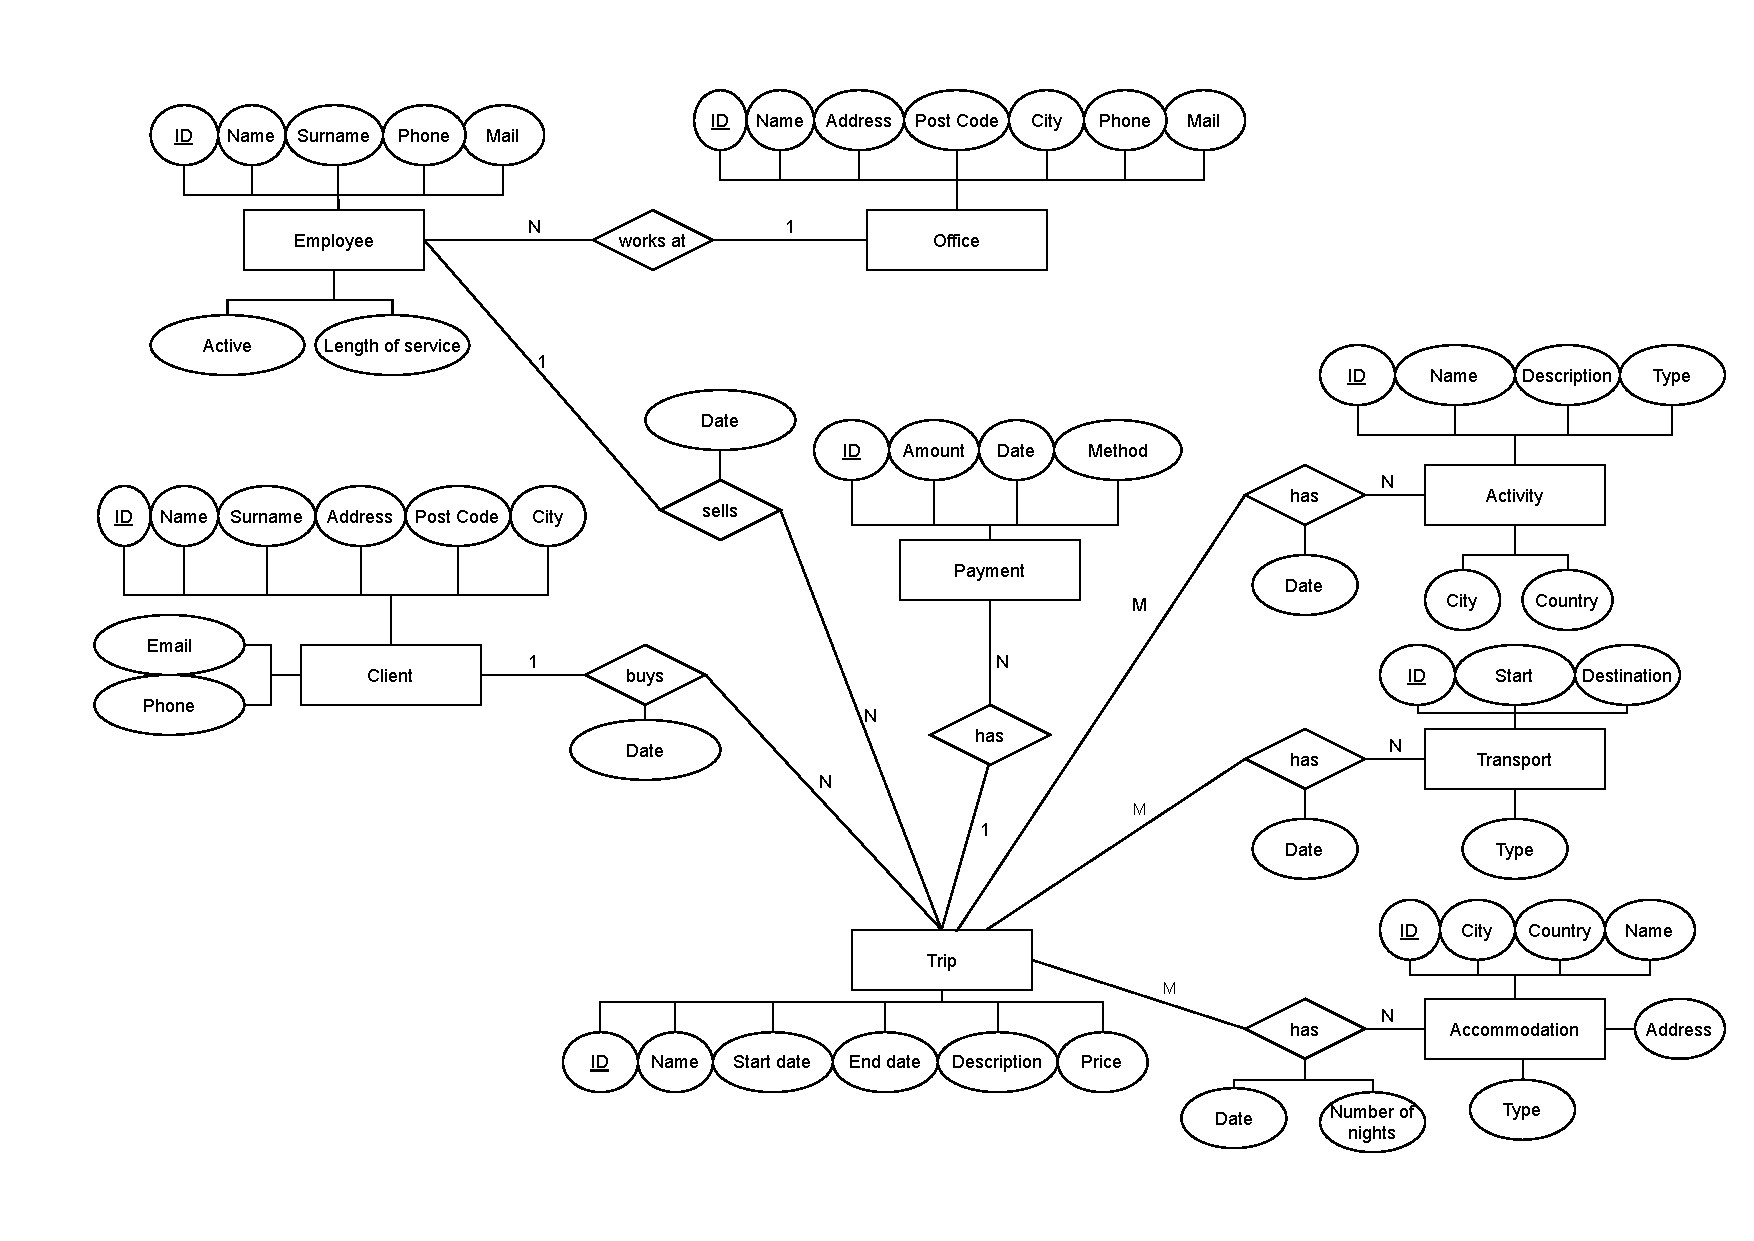
\includegraphics[width=1.15\textwidth, angle=90]{../Diagramm.pdf}
		\label{ER-Model}
		\caption{Travel agency ER-Diagram}
	\end{figure}
	

\end{document}